\section{History}

This package was born out of a $\approx$~10 line function I wrote to estimate the in-core size of a dense matrix (of double precision values).  I need this in my life by a surprising amount, so it made sense to actually create this thing instead of constantly doing ad hoc multiplications of $nrows\times ncols \times 8$ then dividing by powers of $1024$.

But then I got the great idea to make this application $\sim$~enterprise ready~$\sim$ by adding a lot of unnecessary and convoluted OOP.



\section{License}

\begin{figure}[th]
  \centering
  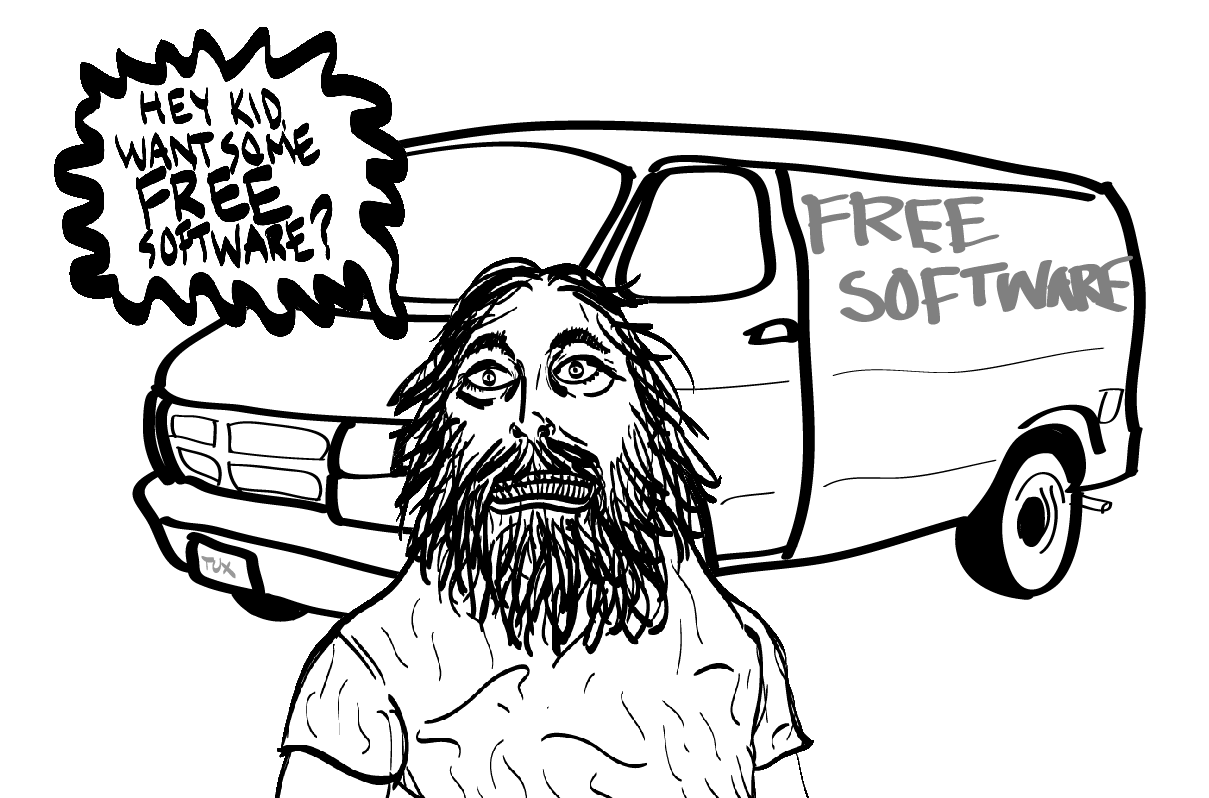
\includegraphics[scale=.35]{./include/gpl.png}
  \caption{The GNU GPL Explained}
  \label{fig:gnu}
\end{figure}
This package is licensed under the GNU General Public License, version $\geq$ 2 (see Figure~\ref{fig:gnu}).
If you violate the terms of the GPL then Richard Stallman's beard will sue you in internet court.


